% !TEX root = ../lab2_report.tex
% ═══════════════════════════════════════════════════════════════
% 实验三：进气畸变条件压气机性能实验
% ═══════════════════════════════════════════════════════════════

\section{实验三：进气畸变条件压气机性能实验}

\subsection{实验目的}

\begin{enumerate}
    \item 了解进气畸变对压气机性能的影响。
    \item 掌握畸变流场的评价指标和测量方法。
    \item 通过与实验一对比，分析畸变进气对压气机稳态特性的影响。
\end{enumerate}

\subsection{实验原理}

在理想状态下，航空发动机压气机进口截面流动均匀。在实际飞行中，当飞机处于大迎角飞行、导弹发射吞烟等情况下，压气机进口会产生严重的不均匀流动——进气畸变。进气畸变是诱发压气机内部流动失稳的关键因素之一。

本实验通过在进口加装畸变发生器（插板），研究畸变进气条件下压气机的稳态特性。受实验条件限制，本批次实验仅使用一种畸变片进行测量。通过与实验一（无畸变）的数据对比，分析畸变对压气机增压能力和失稳边界的影响。

\subsection{实验装置}

\begin{itemize}
    \item 两级低速轴流对转压气机实验台（同实验一）
    \item 畸变发生器（插板）
    \item 稳态参数测量系统
    \item 节流锥控制系统
\end{itemize}

\subsection{实验步骤}

\begin{enumerate}
    \item 停机，更换进气流量管机匣段，安装畸变发生器插板。
    \item 读取并记录大气温度 $T_{\text{atm}}$、大气压力 $P_{\text{atm}}$。
    \item 重新启动压气机，加速到目标转速并等待稳定。
    \item 调节节流锥从全开位置（90\textdegree{}）逐次关小至近失速位置（15\textdegree{}），共记录8个工况点。
    \item 改变转速组合，重复步骤3--4。
    \item 实验结束：停止变频器，关闭所有程序，拆除畸变插板。
\end{enumerate}

\subsection{数据处理方法}

同实验一。

\subsection{实验组别}

为与实验一（无畸变）对比，本实验采用与实验一相同的两组转速组合：

\begin{itemize}
    \item \textbf{组1}：前转子 30 Hz (1800 rpm)，后转子 35 Hz (2100 rpm)，$T_{\text{atm}}=23.7$\textdegree C，$P_{\text{atm}}=96052$ Pa
    \item \textbf{组2}：前转子 28 Hz (1680 rpm)，后转子 37 Hz (2220 rpm)，$T_{\text{atm}}=23.8$\textdegree C，$P_{\text{atm}}=96096$ Pa
\end{itemize}

原始数据文件：\texttt{data/2608xin-J.dat}、\texttt{data/2608（2）xin-J.dat}。

\subsection{数据处理结果及分析}

\subsubsection{畸变进气实验数据}

\begin{table}[H]
  \centering
  \caption{组1 稳态特性数据——前转子1800rpm, 后转子2100rpm（加畸变片） (T=25.374°C, P=95626.0Pa)}
  \label{tab:组1}
  \small
  \setlength{\tabcolsep}{4pt}
  \resizebox{\textwidth}{!}{
    \begin{tabular}{ccccccc}
      \toprule
      节流阀角度° & 进口总压 (Pa) & 进口静压 (Pa) & 出口总压 (Pa) & 出口静压 (Pa) & 总压升 (Pa) & 质量流量 (kg/s) \\
      \midrule
      90.0 & 95624 & 95450 & 95693 & 95577 & 69 & 3.920 \\
      60.0 & 95643 & 95482 & 95750 & 95650 & 107 & 3.827 \\
      50.0 & 95650 & 95486 & 95820 & 95722 & 170 & 3.778 \\
      40.0 & 95620 & 95475 & 95957 & 95871 & 337 & 3.583 \\
      30.0 & 95611 & 95486 & 96200 & 96134 & 589 & 3.324 \\
      25.0 & 95658 & 95543 & 96416 & 96347 & 758 & 3.143 \\
      20.0 & 95649 & 95562 & 96568 & 96517 & 919 & 2.758 \\
      15.0 & 95644 & 95598 & 96534 & 96512 & 890 & 2.037 \\
      \bottomrule
    \end{tabular}
  }
\end{table}

\begin{table}[H]
  \centering
  \caption{组2 稳态特性数据——前转子1680rpm, 后转子2220rpm（加畸变片） (T=25.408°C, P=95646.0Pa)}
  \label{tab:组2}
  \small
  \setlength{\tabcolsep}{4pt}
  \resizebox{\textwidth}{!}{
    \begin{tabular}{ccccccc}
      \toprule
      节流阀角度° & 进口总压 (Pa) & 进口静压 (Pa) & 出口总压 (Pa) & 出口静压 (Pa) & 总压升 (Pa) & 质量流量 (kg/s) \\
      \midrule
      90.0 & 95642 & 95478 & 95704 & 95618 & 62 & 3.829 \\
      60.0 & 95632 & 95465 & 95720 & 95632 & 88 & 3.819 \\
      50.0 & 95636 & 95478 & 95795 & 95715 & 159 & 3.717 \\
      40.0 & 95625 & 95488 & 95951 & 95874 & 326 & 3.554 \\
      30.0 & 95627 & 95502 & 96172 & 96097 & 545 & 3.283 \\
      25.0 & 95672 & 95562 & 96383 & 96321 & 711 & 3.111 \\
      20.0 & 95640 & 95558 & 96504 & 96457 & 864 & 2.716 \\
      15.0 & 95643 & 95592 & 96514 & 96506 & 871 & 2.163 \\
      \bottomrule
    \end{tabular}
  }
\end{table}

\subsubsection{畸变进气特性曲线}

\begin{figure}[H]
    \centering
    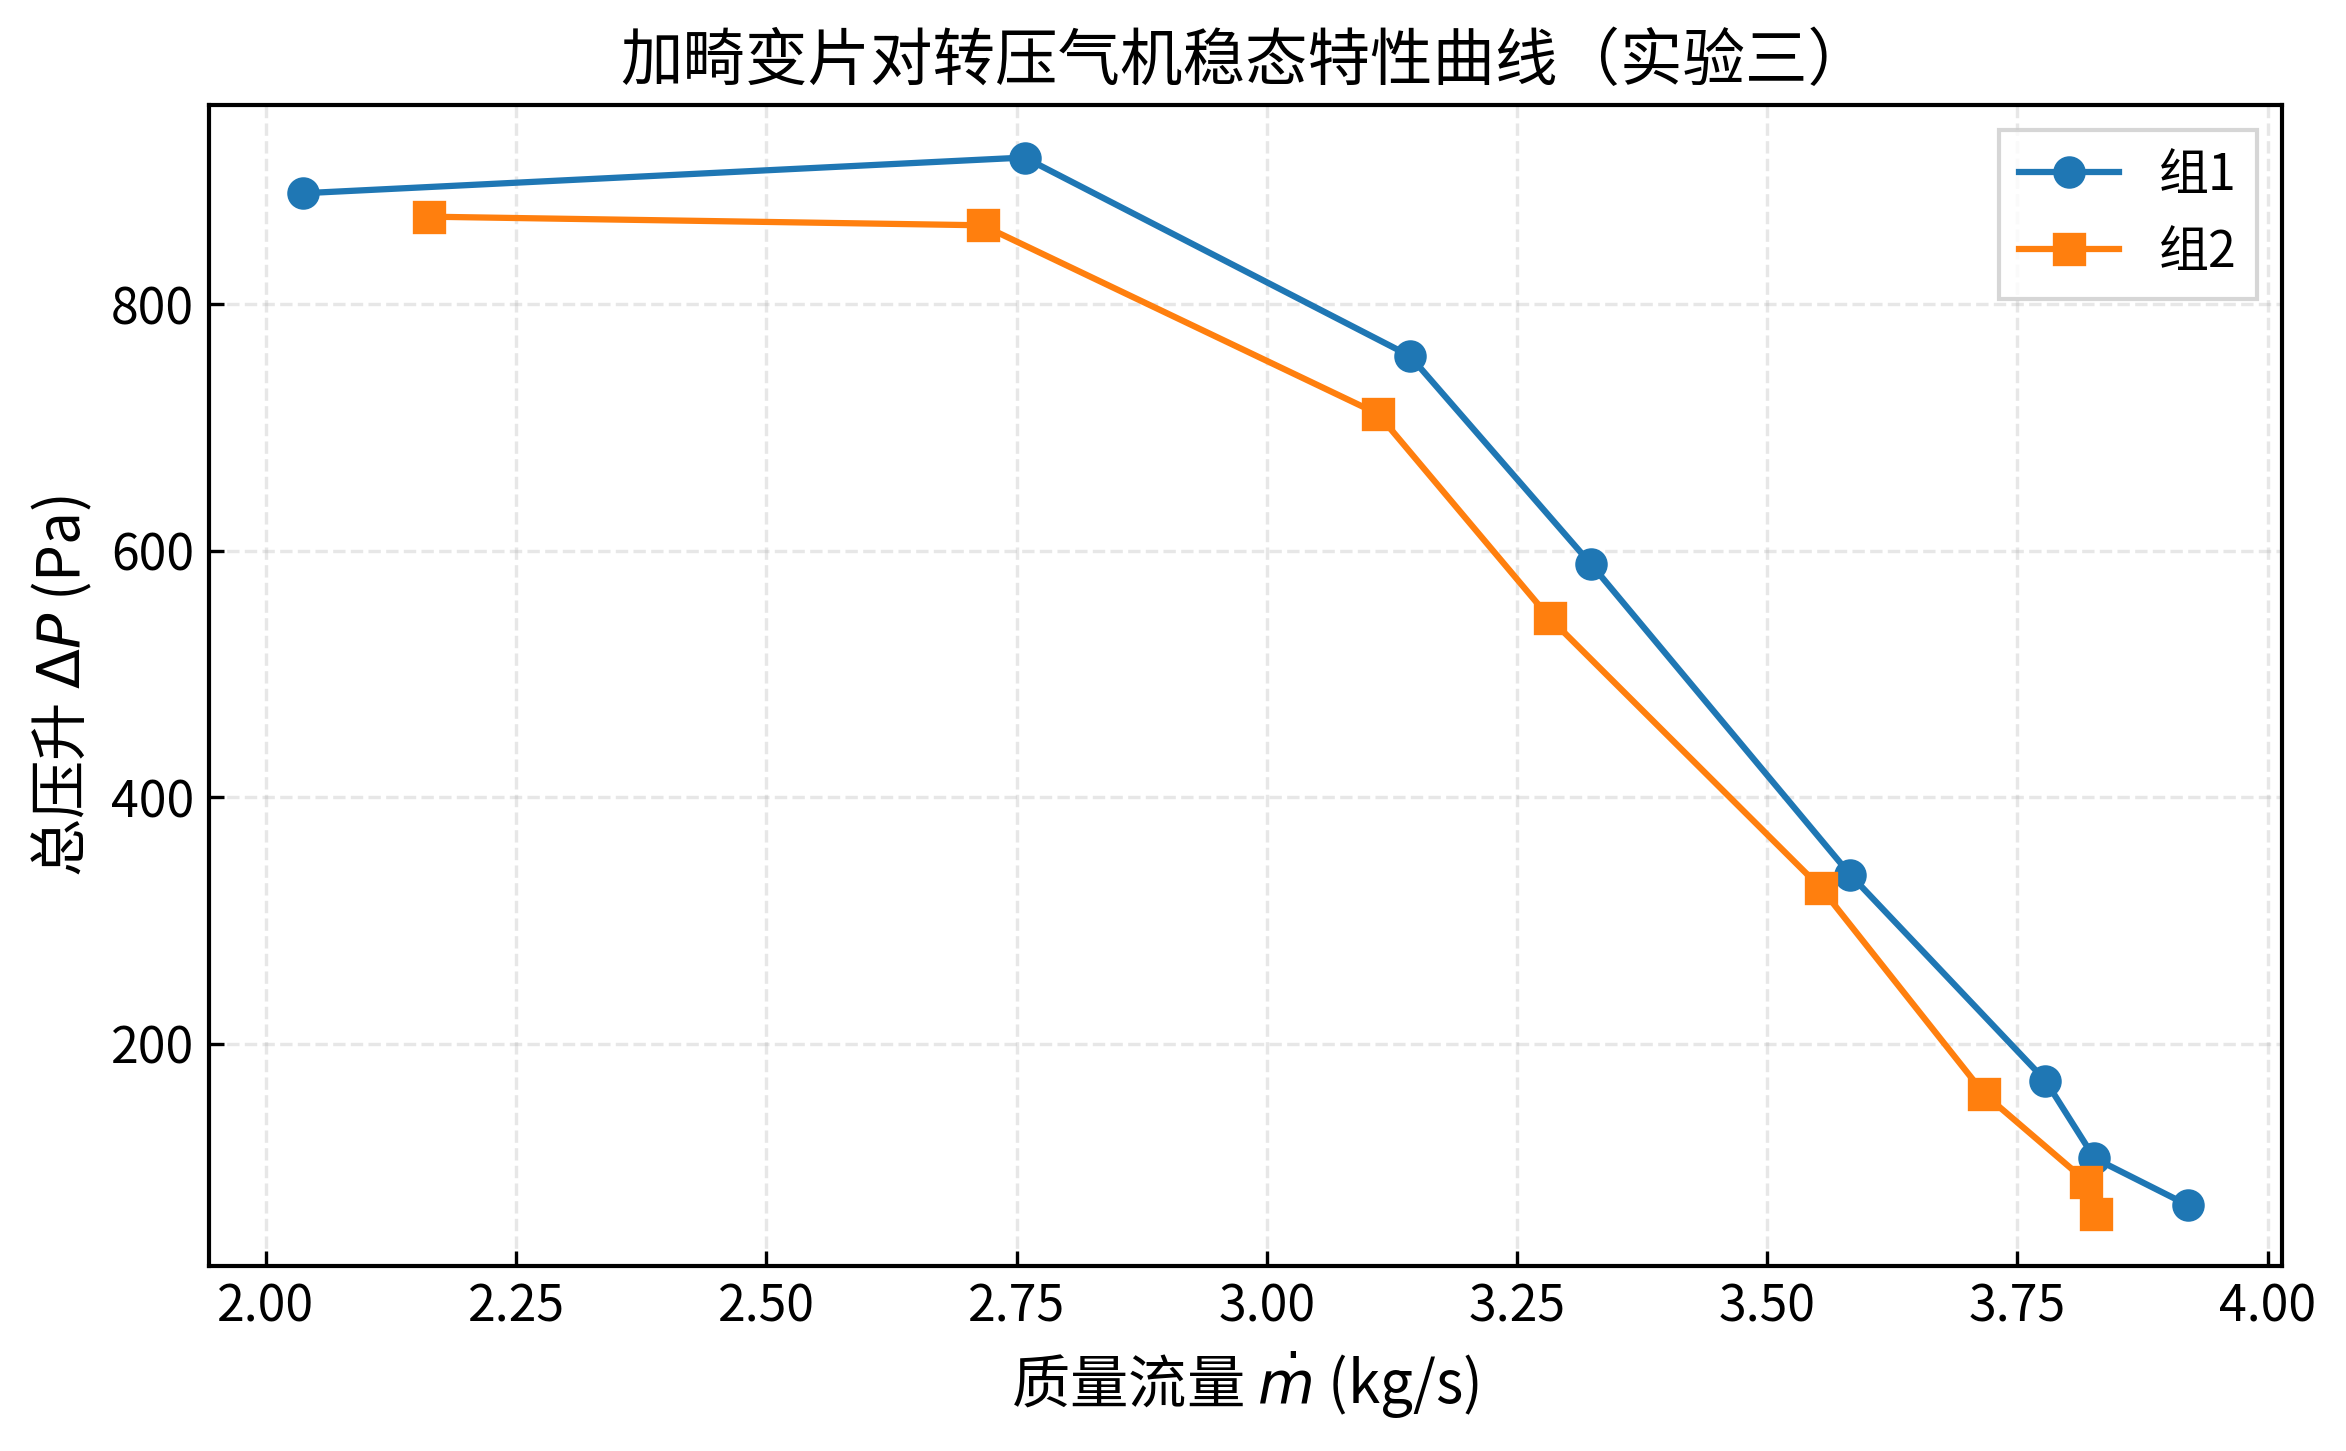
\includegraphics[width=0.85\textwidth]{figures/exp3_characteristics.png}
    \caption{加畸变片条件下两组转速组合的压气机稳态特性}
    \label{fig:exp3}
\end{figure}

\subsubsection{无畸变与加畸变对比}

\begin{figure}[H]
    \centering
    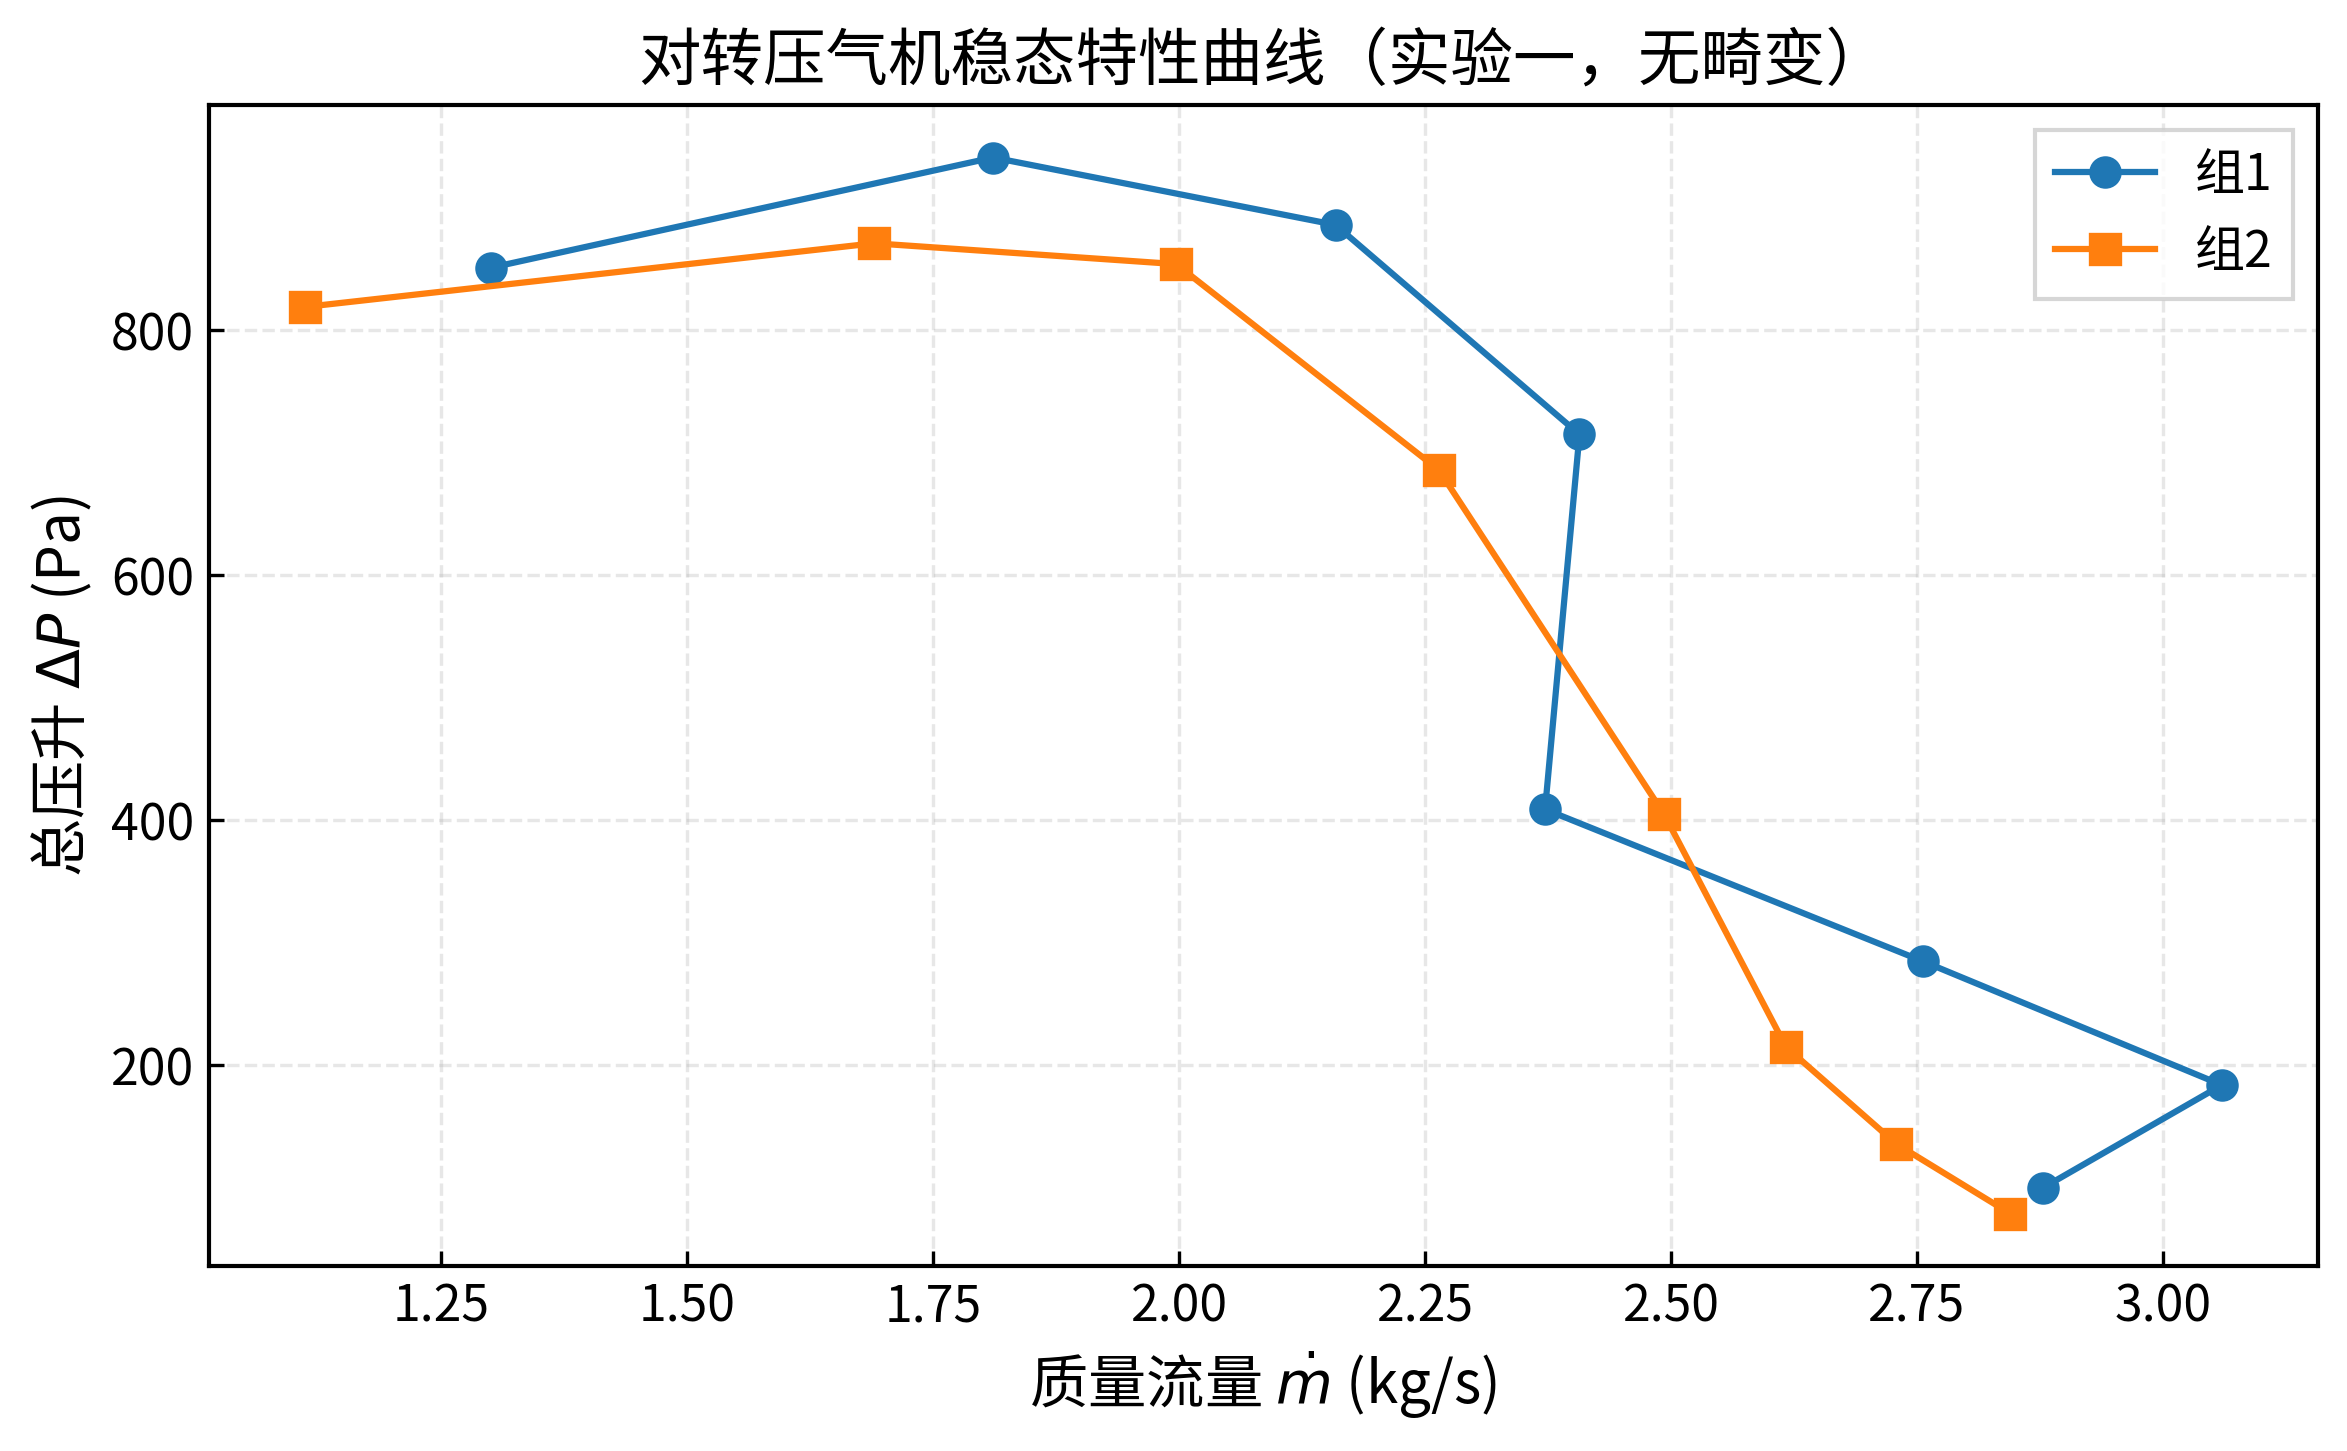
\includegraphics[width=0.85\textwidth]{figures/exp1_2608_characteristics.png}
    \caption{无畸变条件下两组转速组合的压气机稳态特性（实验一，同图~\ref{fig:2608}）}
    \label{fig:exp3_exp1}
\end{figure}

图~\ref{fig:exp3} 和图~\ref{fig:exp3_exp1} 分别展示了加畸变片和无畸变条件下的压气机稳态特性。

\subsubsection{结果分析}

\begin{enumerate}
    \item \textbf{畸变对总压升的影响}：加畸变片后，两组转速组合的总压升均有明显下降。畸变片产生的周向不均匀进气使部分叶片通道始终处于不利来流状态，有效攻角偏离设计值，导致整体增压能力降低。

    \item \textbf{节流特性的一致性}：加畸变后，随着节流角从90\textdegree{}减小到15\textdegree{}，质量流量仍呈单调下降趋势，总压升先增大后趋于平缓，在近失速点（15\textdegree{}）出现拐点。这些基本规律与实验一无畸变条件一致，表明畸变虽降低性能参数的绝对值，但不改变压气机的节流特性规律。

    \item \textbf{失稳边界的影响}：加畸变片后压气机在更高流量下即出现总压升下降，失稳边界向大流量方向移动，稳定工作范围有所缩小。畸变进口使压气机对节流的容忍度降低。

    \item \textbf{转速匹配的影响}：在畸变进气条件下，组1（前后转速差较小）的总压升仍高于组2（前后转速差较大），这与实验一中观察到的趋势一致，说明合理的前后转速匹配即使在畸变条件下也能发挥作用。
\end{enumerate}

\subsection{结论}

在加装一种畸变片的条件下，测量了与实验一相同两组转速组合下的压气机稳态特性，并与实验一的无畸变数据进行对比。实验结果表明进气畸变导致总压升降低，但对压气机的基本节流特性和转速匹配规律没有本质改变。本实验仅使用了一种畸变片，不同畸变形式和程度对压气机特性的影响有待后续实验进一步研究。
